\documentclass[10pt,oneside]{article}
\usepackage{amsmath} % Refined math symbols
\usepackage{graphicx} % Images
\usepackage{subcaption} % The hability of using subfigures
\usepackage{amsfonts}
\usepackage{amssymb} % To use the symbols for numerical sets

% Language options (we set two languages in this text)
\usepackage{polyglossia}
\setmainlanguage[variant=american]{english}
\setotherlanguage{spanish}

% New bibliography system: biber (No bibtex needed)
\usepackage[
  backend=biber
]{biblatex}
\addbibresource{biblio.bib}

%Set the margins and papersize
\usepackage[
  letterpaper,
  left=1cm,
  right=1cm,
  top=1.5cm,
  bottom=1.5cm
]{geometry}

% custom links and pdf metadata
\usepackage[
  final,
  unicode,
  colorlinks=true,
  citecolor=blue,
  linkcolor=blue,
  plainpages=false,
  urlcolor=blue,
  pdfpagelabels=true,
  pdfsubject={Study Notes for Coding Interview},
  pdfauthor={Jorge Antonio García Galicia},
  pdftitle={StudyNotes},
  pdfkeywords={Google, Nvidia, code, interview, codding}
]{hyperref}

%Profesionall looking tables
\usepackage{booktabs}

%To insert algorithms in pseudocode
\usepackage{algpseudocode}
\usepackage{algorithm} %float enviroment for algorithms
%Make the comments similar to cpp
%\algrenewcommand{\algorithmiccomment}[1]{\hskip3em$//$ #1}

%Headers and footers
\usepackage{lastpage}
\usepackage{fancyhdr}
\fancyhf{}
\pagestyle{fancy}
\fancyhf{}
\fancyhead[L]{Study Notes for Coding Interview}
\fancyhead[C]{Jorge Antonio Garc\'ia Galicia} %There is no utf8 in fancyhdr
\fancyhead[R]{\href{mailto:nemediano@gmail.com}{nemediano@gmail.com}}
% https://tex.stackexchange.com/questions/227/how-can-i-add-page-of-on-my-document
\fancyfoot[C]{\thepage\ of \pageref*{LastPage}}
%\fancyfoot[C]{ of }
\renewcommand{\headrulewidth}{2pt} 
\renewcommand{\footrulewidth}{2pt}

\usepackage{minted} %For inserting source code and embed source files
%Requieres compilation using:
% $xelatex -shell-escape input.tex

%In order to work this temple needs to be build like this:
% 1 XeLaTeX
% 2 Biber 
%    This tool is not in the default Kile: I need to install the package and then configure 
%    here: https://tex.stackexchange.com/questions/154751/biblatex-with-biber-configuring-my-editor-to-avoid-undefined-citations/154763#154763)
% 3 XeLaTex
% 4 XeLateX
% 5 ViewPDF

\author{Jorge Antonio Garc\'ia Galicia} % Again, no utf8 I do not know why
\title{Study Notes}
\date{\today}

\usepackage{csquotes} % Because if is not present HERE polyglossia throws a warning

\begin{document}
\maketitle
\thispagestyle{fancy} %So, the title page has fancyheders
%Actual homework in this file
\section{Memory flatenig}

A common problem in multidimensional data situations is memory layout representation. Internally, computers always represent memory in a linear fashion, the idea of \emph{mutidimensional array} it's just sugar syntax added by high level programming lenguajes.

\subsection{One dimensional array}

Given said that, sometimes allocations for such constructs can become dificult to use or declare by themselves. Especially in C++. Lets see an example:

{\centering
\begin{minipage}{\linewidth}
  \begin{listing}[H]
  \inputminted[
  xleftmargin=1.5cm,  %without this option line number goes wrong
  %frame=lines,
  framesep=0.5cm,
  baselinestretch=1.2,
  %fontsize=\footnotesize,
  linenos,
  firstline=15, %If you omit this two fields, the whole file is pulled
  lastline=21
  ]{cpp}{src/ArrayDimensions.cpp}
  \caption{One dimensioal array (by means of \mintinline{cpp}{std::vector} class) used}
  \label{lst:1Dexample}
  \end{listing}
\end{minipage}
\par
}
\vspace{0.5cm}
So far, everything looks good, sintax is clear, braket operator is helping us.
Conceptually, we have a series of variables with the same type that live in a contiguos space in memory. See figure~\ref{fig:1D}.

\begin{figure}[htp]
  \centering
  \begin{subfigure}[b]{0.35\textwidth}
    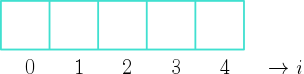
\includegraphics[width=\textwidth]{img/array1D}
    \caption{Logical memory layout representation.}
  \label{fig:1a}
  \end{subfigure}
  \hspace*{4cm}
  \begin{subfigure}[b]{0.25\textwidth}
    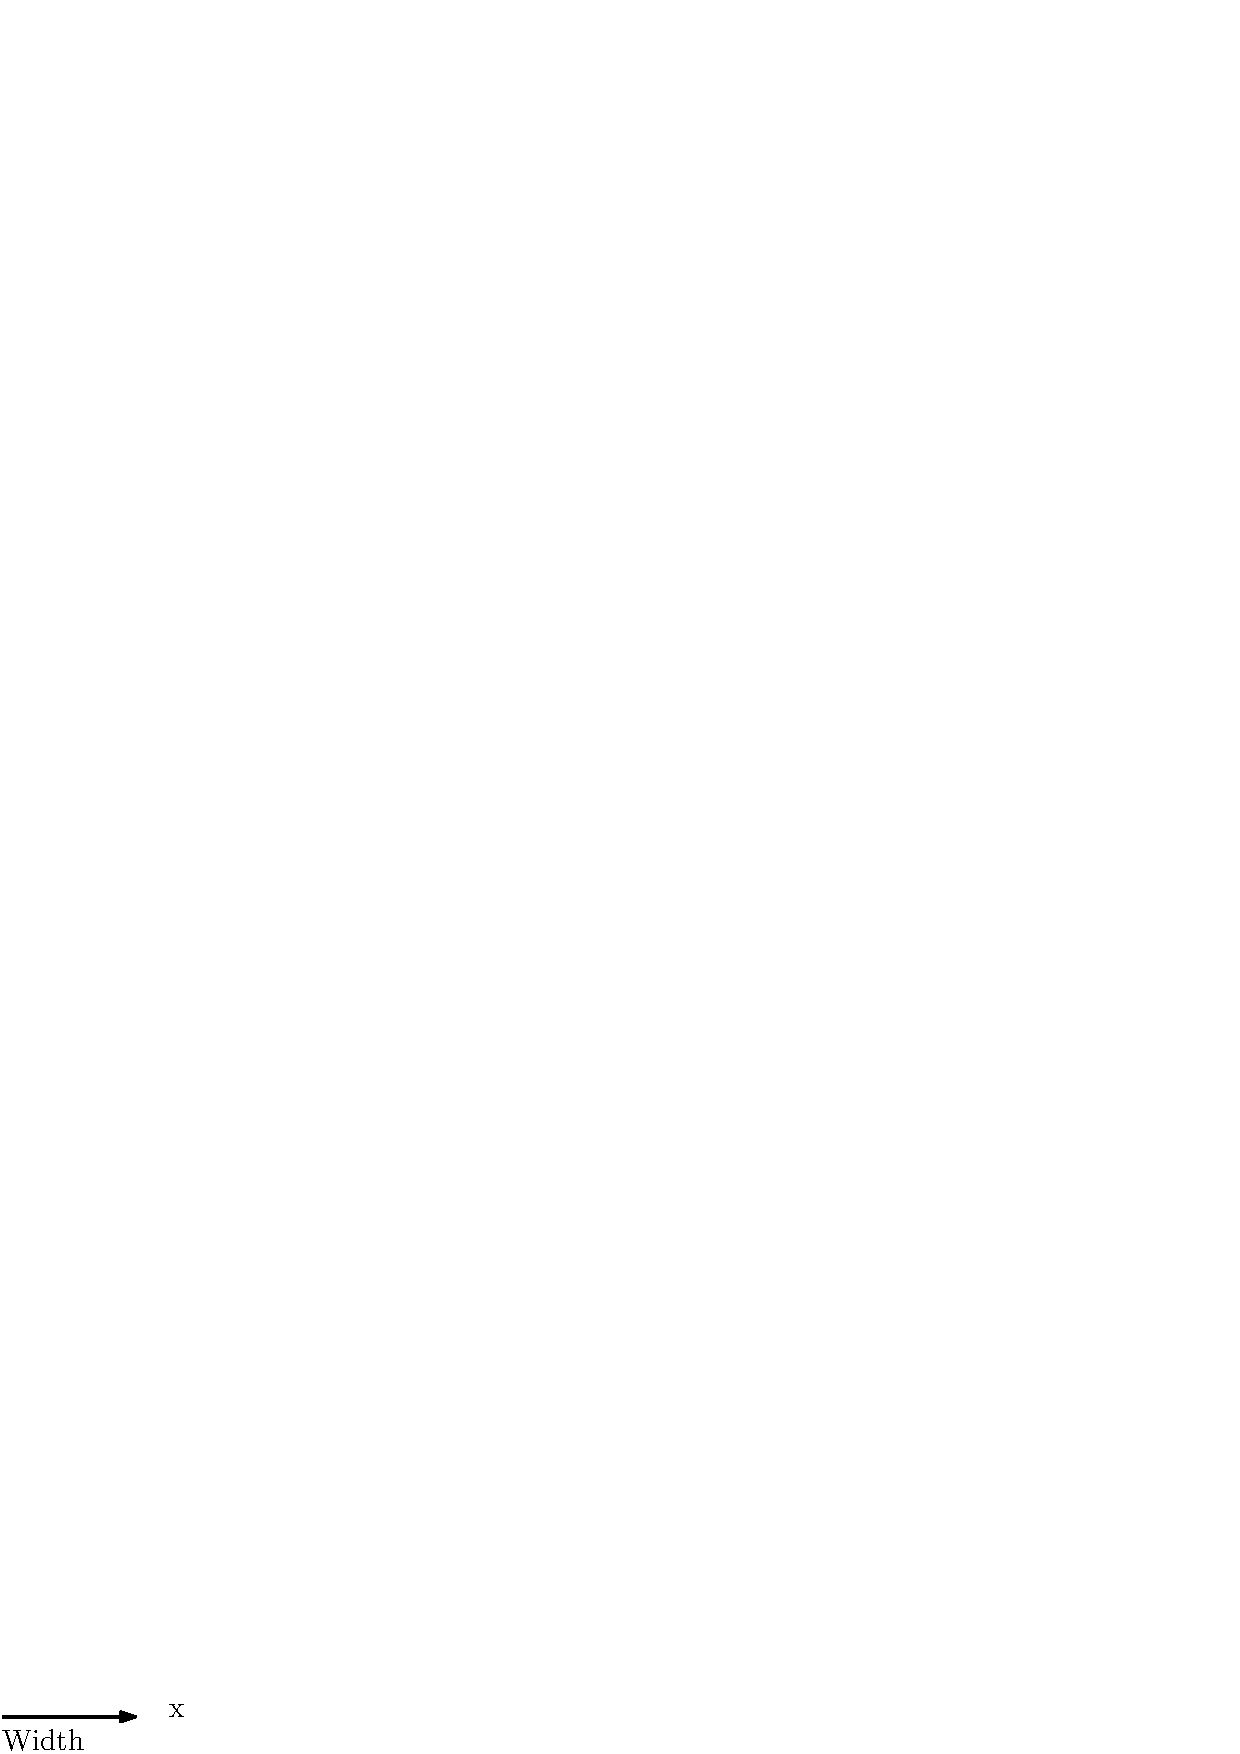
\includegraphics[width=\textwidth]{img/arrow1D}
    \caption{Dimensions represented.}
    \label{fig:1b}
  \end{subfigure}
  \caption{One dimensional array representation.}
  \label{fig:1D}
\end{figure}

\subsection{Two dimensional data}

The problem becomes evident as data start to include more dimensions.
In a bidimensional array we have data that has two dimensions.
One can think about it, like the data it's stored in a table, the situation is the one depicted in Figure~\ref{fig:2a}.
Now, remember this is just an abstraction (provided by our programming language: C++; in this case), since memory is actually \emph{close} to linear in a computer.

\begin{figure}[htp]
  \centering
  \begin{subfigure}[b]{0.35\textwidth}
    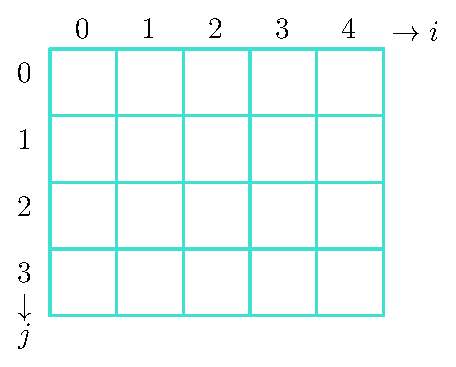
\includegraphics[width=\textwidth]{img/array2D}
    \caption{Logical memory layout representation.}
  \label{fig:2a}
  \end{subfigure}
  \hspace*{4cm}
  \begin{subfigure}[b]{0.25\textwidth}
    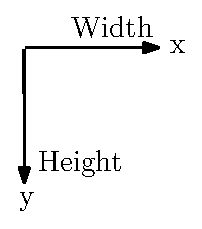
\includegraphics[width=\textwidth]{img/arrow2D}
    \caption{Dimensions represented.}
    \label{fig:2b}
  \end{subfigure}
  \caption{Two dimensional array representation.}
  \label{fig:2D}
\end{figure}

Usually, the C++ way of modeling this is creating an array, such that each element of it, is also an array. See the code in Listing~\ref{lst:2dexample}

{\centering
\begin{minipage}{\linewidth}
  \begin{listing}[H]
  \inputminted[
  xleftmargin=1.5cm,  %without this option line number goes wrong
  %frame=lines,
  framesep=0.5cm,
  baselinestretch=1.2,
  %fontsize=\footnotesize,
  linenos,
  firstline=23, %If you omit this two fields, the whole file is pulled
  lastline=38
  ]{cpp}{src/ArrayDimensions.cpp}
  \caption{Two dimensioal array example}
  \label{lst:2dexample}
  \end{listing}
\end{minipage}
\par
}
\vspace{0.5cm}
Now, there is three main points to highlight in the sample:
\begin{enumerate}

\item The type of the array has change.
      Now is \emph{a vector of int vectors}.
      This led us to have a longer initialization for it too.
      Imagine that you create functions to receive or return such arrays.
      The sintax to declare the parameters become difficult.

\item We still have the advantage of a very elegant sintax to use the array:  \mintinline{cpp}{b[j][i]} give us the element on column $i$ of row $j$.

\item The sintax is backwads with respect to mathematic representation.
      See Figure~\ref{fig:2D} again.
      The index \mintinline{cpp}{i} is transversin along the $x$ dimension and the index \mintinline{cpp}{j} along the $y$ dimension.
      Therefore, the element \mintinline{cpp}{b[j][i]} it's close to $b(x, y)$ in math
 \end{enumerate}

\subsection{Memory flatenig explained}

Here is when the technique called \emph{memory flattening} becomes useful.
In simple words: This is to mimic what the compiler is doing for us: use linear data.
But at the same time you also provide an abstraction, so you can access it in a similar fashion that if your data had more dimensions.
In other works you simulate the access via indices for all the simulated dimensions.

See the Figure~\ref{fig:Flat}.
The data is equivalent to the one shown in Figure~\ref{fig:2D} in the sense that represents a two dimensional table, whose first dimension $x$ (number of columns: $5$), indexed by $i \in \{0, 1, 2, 3, 4\}$ and whose second dimension $y$ (number of rows: $4$) is indexed by $j \in \{0, 1, 2, 3\}$.
However, the data is stored in a one dimensional array of size $5 \cdot 4 = 20$.
The actual indices of the array go in $0, 1, \ldots, 19$ and are shown on the bottom of of Figure~\ref{fig:Flat}.
However, we also provide an abstraction to access this data via simulated indices \mintinline{cpp}{[j][i]} shown in the top of Figure~\ref{fig:Flat}

\begin{figure}[htb]
  \centering
  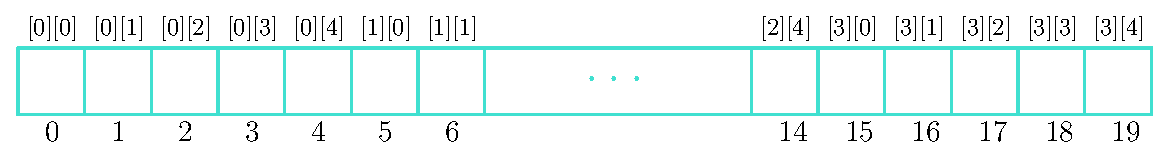
\includegraphics[width=0.85\textwidth]{img/arrayFlat}
  \caption{2D array represented in a flattened array. This represents the same data as Figure~\ref{fig:2D}. Order of the indices is \mintinline{cpp}{[j][i]}}
  \label{fig:Flat}
\end{figure}

This has the advantage that all the data is store in a one dimensional array.
Therefore, you \emph{ensure} all your data is actually contigous in memory.
Also, no matter how many dimensions your data has, the type is always a one dimensional array.
Provided that we acces it in the \emph{same way}, the access tends to be faster than the alternative shown in Listing~\ref{lst:2dexample}
The \emph{same way} means that the inner loop moves along the $x$ dimension and the outer loop transverses the second dimension $y$.
The reason for this improvement becomes evident if we see Figure~\ref{fig:Flat}: in this way, we are actually accesing a linear array in his linear order.

In order to implement this technique we will need two mappings:
First, a function $g:\mathbb{Z}^n \rightarrow \mathbb{Z}$, to map the indices in $n$ dimensions to the one dimensional array.
And second, the inverse mapping $h:\mathbb{Z} \rightarrow \mathbb{Z}^n$ to retrive the indices back given a position in the data buffer.

The first function $g$ it is actually the most useful to us, since it will provide with the interface of accesing our data.
See the Figure~\ref{fig:2D}.
Assume that our data hast two dimensions ($x$ and $y$ --or \emph{width} and \emph{height}-- if you like).
That we use two indices $i$ and $j$ to transverse it.
And assume also that the maximun values of such indices are \mintinline{cpp}{WIDTH} and \mintinline{cpp}{HEIGHT} and that they are zero based.
In Listing~\ref{lst:functions2D} we show the implementation of such function.

We can see that the transformations are actually very simple.
In fact, one of them is the integer division and the other one is the modulo.
Also note, that as long as we check for the boundaries of the values for both indices, only one of the maximun dimensions in this case \emph{witdh} is used in the actual calculation of the indices.

{\centering
\begin{minipage}{\linewidth}
  \begin{listing}[H]
  \inputminted[
  xleftmargin=1.5cm,  %without this option line number goes wrong
  %frame=lines,
  framesep=0.5cm,
  baselinestretch=1.2,
  %fontsize=\footnotesize,
  linenos,
  firstline=86, %If you omit this two fields, the whole file is pulled
  lastline=103
  ]{cpp}{src/FlatMemmory.cpp}
  \caption{Function $g$ to map real index into simulated 2D indices}
  \label{lst:functions2D}
  \end{listing}
\end{minipage}
\par
}
\vspace{0.5cm}

For completeness, we also show Listing~\ref{lst:functions2D2} that defines the inverse function $h$, to retrive the index in the one dimensional array from the two simulated indices in 2D.

{\centering
\begin{minipage}{\linewidth}
  \begin{listing}[H]
  \inputminted[
  xleftmargin=1.5cm,  %without this option line number goes wrong
  %frame=lines,
  framesep=0.5cm,
  baselinestretch=1.2,
  %fontsize=\footnotesize,
  linenos,
  firstline=105, %If you omit this two fields, the whole file is pulled
  lastline=119
  ]{cpp}{src/FlatMemmory.cpp}
  \caption{Function $h$ to map simulated 2D indices into the real index, this is the inverse of $g$}
  \label{lst:functions2D2}
  \end{listing}
\end{minipage}
\par
}
\vspace{0.5cm}

\subsection{Three dimensional data}

Now, lets look at the more complex --but still very common-- scenario of three dimensions. The situation is the one depicted in Figure~\ref{fig:3D}. We include a new dimension in the data: indexed by $k$ along the $z$ axis, we call it \emph{depth}.

\begin{figure}[htp]
  \centering
  \begin{subfigure}[b]{0.35\textwidth}
    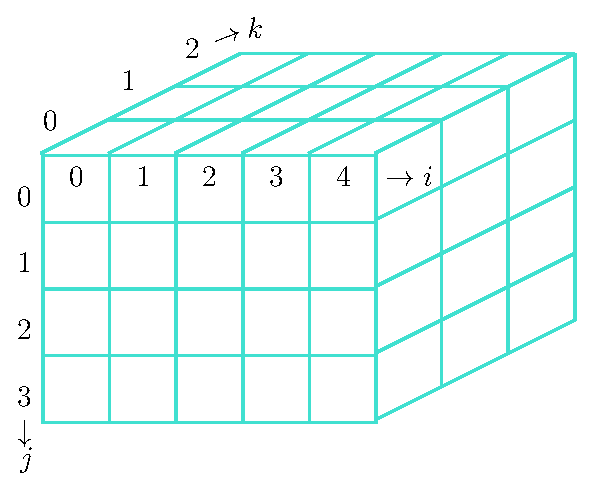
\includegraphics[width=\textwidth]{img/array3D}
    \caption{Logical memory layout representation.}
  \label{fig:3a}
  \end{subfigure}
  \hspace*{4cm}
  \begin{subfigure}[b]{0.2\textwidth}
    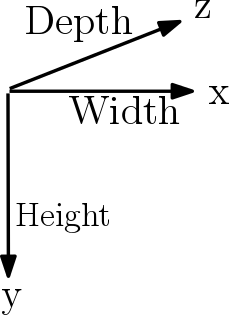
\includegraphics[width=\textwidth]{img/arrow3D}
    \caption{Dimensions represented.}
    \label{fig:3b}
  \end{subfigure}
  \caption{Three dimensional array representation.}
  \label{fig:3D}
\end{figure}

In the normal mutidimensional array synatx C++ syntax this will become, an array of arrays of array of ints. See Listing~\ref{lst:3dexample}. We transvers it using three nested loops, where the most outer one is the one indexed by the new dimension.

{\centering
\begin{minipage}{\linewidth}
  \begin{listing}[H]
  \inputminted[
  xleftmargin=1.5cm,  %without this option line number goes wrong
  %frame=lines,
  framesep=0.5cm,
  baselinestretch=1.2,
  %fontsize=\footnotesize,
  linenos,
  firstline=40, %If you omit this two fields, the whole file is pulled
  lastline=64
  ]{cpp}{src/ArrayDimensions.cpp}
  \caption{Three dimensional array example in C++}
  \label{lst:3dexample}
  \end{listing}
\end{minipage}
\par
}
\vspace{0.5cm}

For memory flatening, we will need new functions $g$ and $h$, that depends in a new extra parameter: \mintinline{cpp}{DEPTH}. In Listing~\ref{lst:functions3D}, we can see the new function $g$.

{\centering
\begin{minipage}{\linewidth}
  \begin{listing}[H]
  \inputminted[
  xleftmargin=1.5cm,  %without this option line number goes wrong
  %frame=lines,
  framesep=0.5cm,
  baselinestretch=1.2,
  fontsize=\footnotesize,
  linenos,
  firstline=121, %If you omit this two fields, the whole file is pulled
  lastline=141
  ]{cpp}{src/FlatMemmory.cpp}
  \caption{New function $g$ to map real index into simulated 3D indices}
  \label{lst:functions3D}
  \end{listing}
\end{minipage}
\par
}
\vspace{0.5cm}

Similarly, the new function $h$ is presented in Listing~\ref{lst:functions3D2}

{\centering
\begin{minipage}{\linewidth}
  \begin{listing}[H]
  \inputminted[
  xleftmargin=1.5cm,  %without this option line number goes wrong
  %frame=lines,
  framesep=0.5cm,
  baselinestretch=1.2,
  fontsize=\footnotesize,
  linenos,
  firstline=143, %If you omit this two fields, the whole file is pulled
  lastline=161
  ]{cpp}{src/FlatMemmory.cpp}
  \caption{A new function $h$ to map simulated 3D indices into the real index, this is the inverse of $g$}
  \label{lst:functions3D2}
  \end{listing}
\end{minipage}
\par
}

\section{Bitwise operation}
\begin{itemize}
  \item Basic operations. Bit vs Byte How to handle printing in C++
  \item One bit manipulation, set, clear, toggle and testing
  \item Bit masking: set, clear, toggle and test group of bites
\end{itemize}

\section{Analytic Geometry}
\begin{itemize}
  \item Ray, line and segment representations
  \item Ray to segment intersection
  \item Projecction
  \item Point to segment distance
  \item Belonging test on simple polygons
\end{itemize}

\section{Graphics Pipeline}
\begin{itemize}
  \item Simple: Vertex and fragment
  \item Complete, all optional stages
  \item Texture pipeline
\end{itemize}

%Add this book to the reference table even if we do not cite explicitly
\nocite{Laakmann2015}
%Add the references
\printbibliography
\end{document}
